\section{研究背景和动机}
\label{chap:hash:motivation}

本节对该方法中涉及的相关背景进行介绍,包括网络噪声对时间隐通道的干扰方式,以及基于码字间校验的鲁棒性策略。其中,网络噪声对时间隐通道的干扰,主要分析了不同类型的网络噪声对码字鉴别的干扰情况,并提出了问题的解决方法。基于码字间检验的鲁棒性策略,提出了建立码字间的校验关系,提高校验信息利用率的方法。

\subsection{网络噪声对时间隐通道的干扰}
\label{chap:hash:motivation:noise}

由图\nref{fig:2:pmf-dropout}可知,VoLTE视频通话中丢包长度为1的突发丢包占比在50\%左右,而其余的均为连续丢包事件。通过CRC检错码等方式,对离散的随机丢包噪声具有较好的抑制作用,而在连续丢包噪声干扰中,数据码字及校验码字出现误匹配概率较高,导致码字鉴别准确率较低,最终传输结果的误码率升高。

\insertFigure{
	\begin{figure}
		\centering
        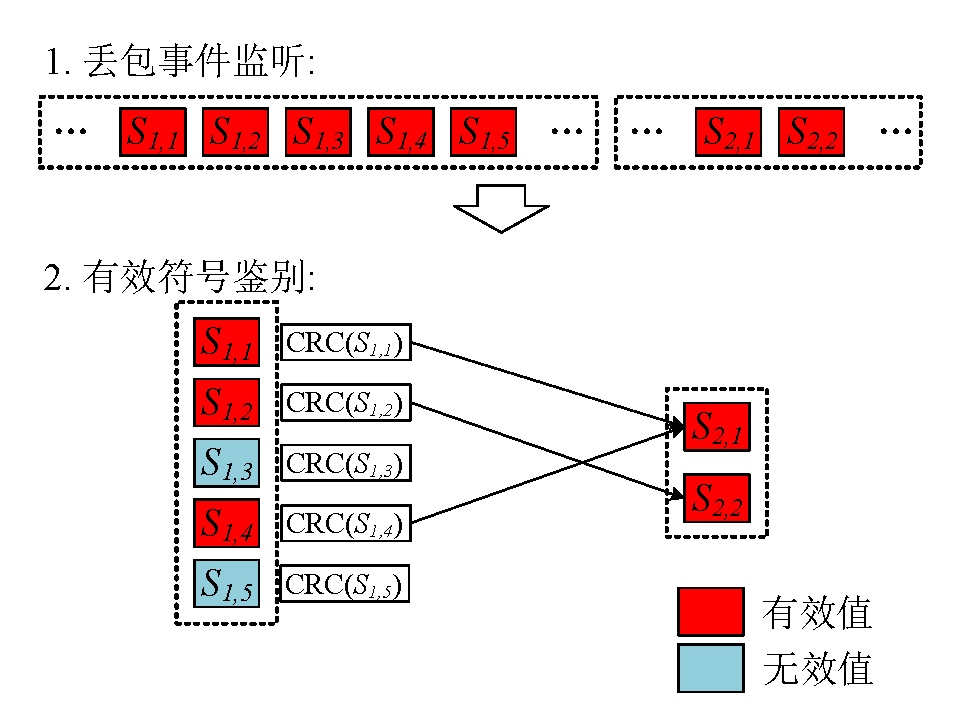
\includegraphics[width=0.7\textwidth]{chapters/chapter5/figures/crc-continuous.pdf}
        \caption{连续丢包对鉴别过程的影响示意图}
        \label{fig:5:crc-continuous}
	\end{figure}
}

如图\nref{fig:5:crc-continuous},存在连读丢包的情况下,通过CRC进行有效符号鉴别,存在明显的校验能力退化。第一组$S_{1}$为待验证的数据符号,第二组$S_{2}$为可能的校验符号,在第一步的丢包事件监听中,无法区分符号的有效性,因此所有的符号作为候选值进入第二步。在有效符号鉴别过程中,依次计算CRC($S_{1,i}$),并将结果与$S_{2,j}$比较,由于校验符号只是CRC散列结果的一部分,存在碰撞的概率较高。最终的鉴别结果,只能识别出部分网络噪声。由于缺乏额外的鉴别信息,无法进一步判别噪声,导致解调结果出现误码。

理想情况下,按照\nref{chap:zigzag:model:modulation:crc}中设计的鲁棒性方案,当数据组出现噪声而校验组无噪声时,产生误码的概率为$1/L_{Codeword}$,具备有效的鉴别能力。而实际场景中,校验组也会受噪声干扰,产生图\nref{fig:5:crc-continuous}中鉴别失效的结果。

\insertFigure{
	\begin{figure}
		\centering
        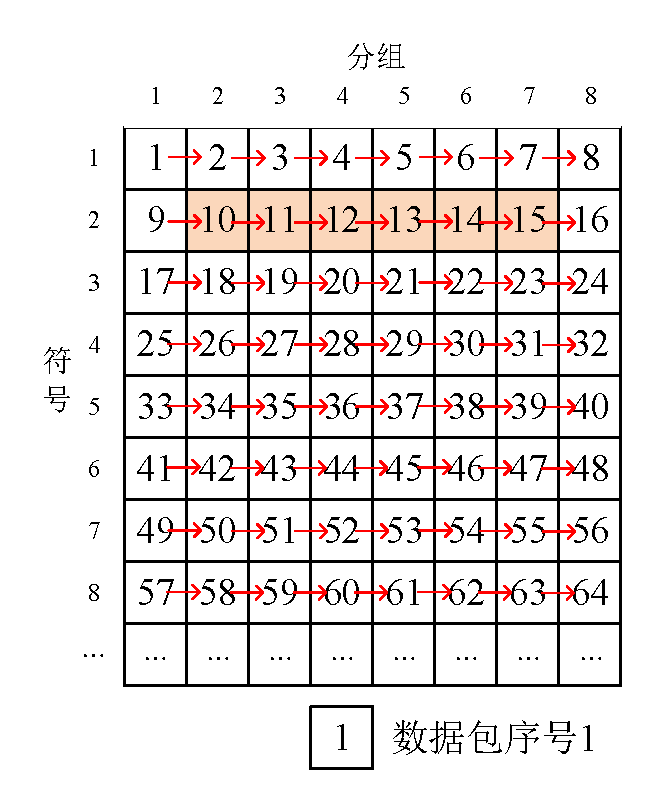
\includegraphics[width=0.45\textwidth]{chapters/chapter5/figures/row-matrix.pdf}
        \caption{符号-数据包序号映射矩阵示意图}
        \label{fig:5:row-matrix}
	\end{figure}
}

在VoLTE视频通话中,丢包时刻存在随机性,出现密集连续丢包的概率较低。因此,将连续丢包导出的符号分散,利用每组的校验能力,降低噪声干扰,是应对该类型噪声的可行办法。如图\nref{fig:5:row-matrix},矩阵中的位置为数据包序号,矩阵元素的列号为组号,行号对应符号。当出现连续丢包,如$10\sim 15$,经过该映射矩阵的处理,被分配到分组$2\sim 7$,有利于充分利用校验字段的校验能力,提高校验资源利用率。

\subsection{基于码字间校验的鲁棒性策略}
\label{chap:hash:motivation:robustness}

时间隐通道的鲁棒性策略中,包含喷泉码等无速率编码,结合多个码字之间的数据冗余,还原真实的消息内容,扩大了校验信息的作用范围。\nupcite{6296078}在区块链技术中,每一个区块中均含有前一个区块的HASH值,因此当链长达到一定规模时,起始区块的正确性越高。\nupcite{7467408}在基于主动丢包的时间隐通道中,由于噪声分布不均匀,添加码字间校验关系,利用低噪声的信息校验高噪声的数据,进一步提高校验信息利用率。

\insertFigure{
	\begin{figure}
		\centering
        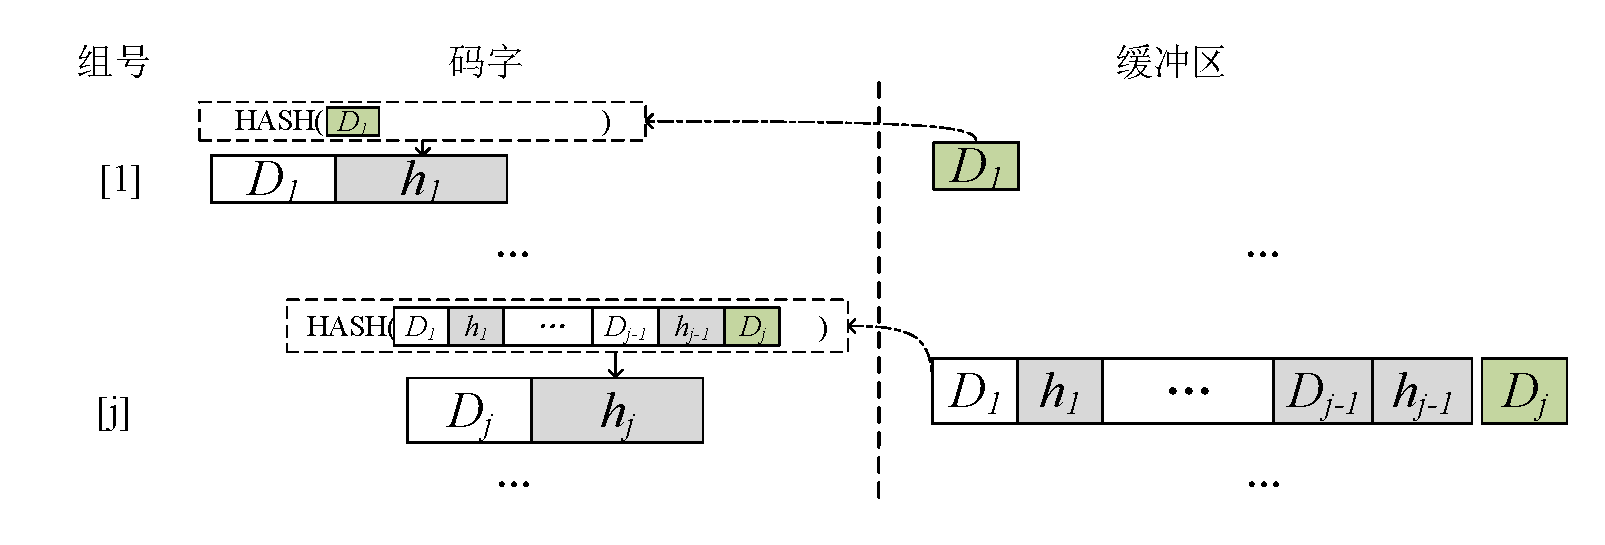
\includegraphics[width=0.95\textwidth]{chapters/chapter5/figures/chain-example.pdf}
        \caption{码字间校验结构示意图}
        \label{fig:5:chain-example}
	\end{figure}
}

如图\nref{fig:5:chain-example},码字间校验块$h_{j}$记录了数据缓冲区的校验结果。借助HASH函数的随机性和确定性,随着接收组数的增长,通过后接收码字中的码字间校验信息,验证已经接收到码字的正确性。即使部分的码字受噪声干扰,借助其它组中的低噪声有效信息,完成码字鉴别,降低噪声干扰强度。

码字间校验的HASH摘要,在计算时进行了加盐处理,通过结合用户自定义信息及RTP随机字段,提高了时间隐通道保密性。监听者监听到丢包事件后,无法正确恢复码字间校验块$h_{j}$,从而无法验证码字间校验关系,存在噪声干扰时无法区分噪声及信号,隐蔽消息得到保护。

\subsection{研究动机}
\label{chap:hash:motivation:motivation}

本时间隐通道构建方法,基本的调制方式为主动丢包,将调制产生的丢包隐匿在网络噪声中,通过多重校验的方式在解调过程中有效去噪,提高鲁棒性降低误码率。在多重校验的基础上,引入加盐及随机化过程,增加调制过程的随机度,增强隐蔽消息的保密性。

\insertFigure{
	\begin{figure}
		\centering
        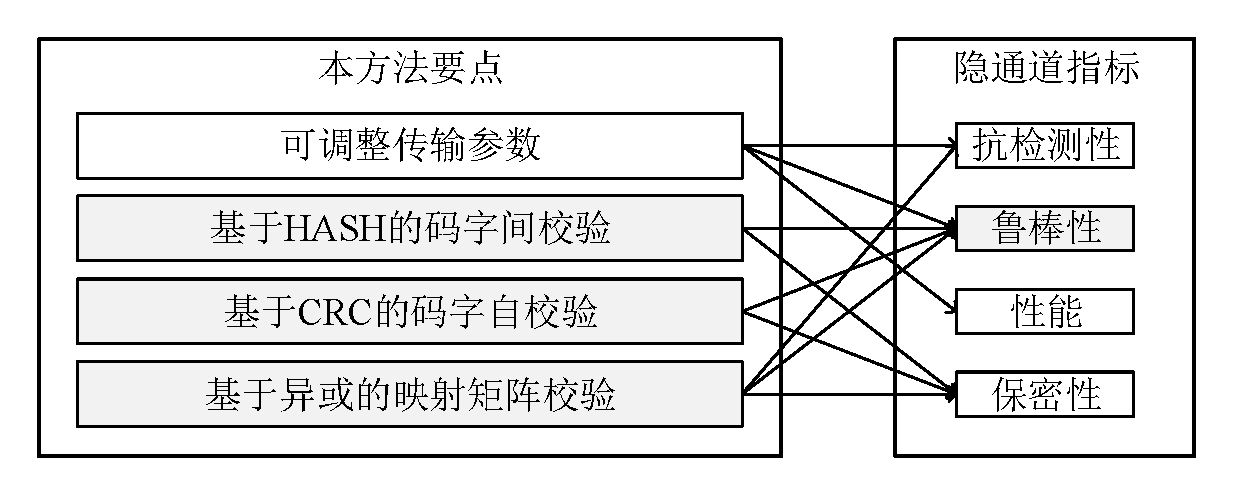
\includegraphics[width=0.8\textwidth]{chapters/chapter5/figures/chapter-struct.pdf}
        \caption{基于多重校验的时间隐通道构建方法研究要点与指标}
        \label{fig:5:chapter-struct}
	\end{figure}
}

如图\nref{fig:5:chapter-struct},本方法的要点主要有可调整传输参数、基于HASH的码字间校验、基于CRC的码字自校验及基于异或的映射矩阵校验。其中,可调整传输参数主要解决抗检测性、鲁棒性及传输性能之间的均衡问题。该方法中需要牺牲性能保证鲁棒性,因此通过调整传输参数实现各方面的统筹。基于HASH的码字间校验、基于CRC的码字自校验,主要提升时间隐通道的鲁棒性,同时提高隐蔽消息的保密性。基于异或的映射矩阵校验,通过构建具有校验能力的映射矩阵,在分散丢包位置的基础上提高鲁棒性。